%TODO: add some references (63, 62, 61, 59, 58) to final sentence
\documentclass[%
%preprint,
 reprint,
superscriptaddress,
%groupedaddress,
%unsortedaddress,
%runinaddress,
%frontmatterverbose,
showpacs,preprintnumbers,
%nofootinbib,
%nobibnotes,
%bibnotes,
 amsmath,amssymb,
 aps,
 prl,
%pra,
%prb,
%rmp,
%prstab,
%prstper,
floatfix,
]{revtex4-1}
\usepackage{natbib}
\usepackage{xcolor}
\usepackage{graphicx}% Include figure files
% \setlength{\intextsep}{0mm}
\usepackage{siunitx}
\usepackage{dcolumn}% Align table columns on decimal point
\usepackage{bm}% bold math
\usepackage{hyperref}% add hypertext capabilities
\usepackage[mathlines]{lineno}% Enable numbering of text and display math
\usepackage{mathtools}
\usepackage[caption=false]{subfig}
\usepackage[percent]{overpic}
% \linenumbers\relax % Commence numbering lines %WARNING: not work with subfig!
\usepackage[mathscr]{euscript}
\graphicspath{{figures/}{.}}

% Copied from mathrsfs.sty
\DeclareSymbolFont{rsfs}{U}{rsfs}{m}{n}
\DeclareSymbolFontAlphabet{\mathscrsfs}{rsfs}

%\usepackage[showframe,%Uncomment any one of the following lines to test
%%scale=0.7, marginratio={1:1, 2:3}, ignoreall,% default settings
%%text={7in,10in},centering,
%%margin=1.5in,
%%total={6.5in,8.75in}, top=1.2in, left=0.9in, includefoot,
%%height=10in,a5paper,hmargin={3cm,0.8in},
%]{geometry}
\DeclareSIUnit\basepair{bp}
%macros
\newcommand{\gwlc}[2][\Omega_0; L_1]{G_\text{\tiny TWLC}(#2|#1)}
\newcommand{\ghat}[2][\Omega_0; L_1]{\hat{G}_\text{\tiny TWLC}(#2|#1)}
\newcommand{\greens}[2][\Omega_0; L]{G(#2|#1)}
%TODO: change path integral D to be different from mathcal (D)
\newcommand{\pathd}[1]{\mathscrsfs{D}\left[#1\right]}
\newcommand{\energy}{\mathcal{E}}
\newcommand{\wigD}{\mathcal{D}}
\newcommand{\RR}{\left\langle{}R^2\right\rangle{}}
\newcommand{\meanli}{\left\langle{}L_i\right\rangle}

\begin{document}
%\preprint{APS/123-QED}
\title{Geometrical Heterogeneity Dominates
Thermal Fluctuations in {\color{red} Facilitating Chromatin Contacts}}%
\author{Bruno Beltran}%
\thanks{These authors contributed equally to this work.}%
\affiliation{%
    Biophysics Program, Stanford University, Stanford, California 94305, USA%
}%
\author{Deepti Kannan}%
\thanks{These authors contributed equally to this work.}%
\author{Quinn MacPherson}%
\affiliation{%
    Department of Physics, Stanford University, Stanford, California 94305, USA%
}%
\author{Andrew J. Spakowitz}%
\email{ajspakow@stanford.edu}%
% \homepage{http://web.stanford.edu/~ajspakow/}%
\affiliation{%
    Chemical Engineering Department, Stanford University, Stanford, California 94305, USA%
}%
\affiliation{%
    Department of Materials Science and Engineering, Stanford University Stanford, California 94305, USA%
}%
\affiliation{%
    Department of Applied Physics, Stanford University, Stanford, CA 94305%
}%
\date{\today}% It is always \today, today,
             %  but any date may be explicitly specified

\begin{abstract}
Within a living cell, the myriad of proteins that bind DNA introduce heterogeneously spaced kinks into an otherwise semiflexible DNA double helix.
To investigate the effects of heterogeneous nucleosome binding on chromatin organization, we extend the wormlike chain (WLC) model to include statistically spaced, rigid kinks.
On time scales where nucleosome positions are fixed, we find that the probability of chromatin loop formation can vary by up to six orders of magnitude between two sets of nucleosome positions drawn from the same distribution.
On longer time scales, we show that continuous re-randomization due to nucleosome turnover results in chromatin tracing out an effective WLC with a dramatically smaller Kuhn length than bare DNA.
Together, these observations {\color{red} demonstrate that nucleosome spacing
    acts as the primary source of the structural heterogeneity that dominates local and global chromatin organization.}
\end{abstract}

% PACS, the Physics and Astronomy Classification Scheme.
\pacs{05.20.--y, 05.40.Fb, 36.20.Ey, 87.10.Ca, 87.14.gk, 87.15--v, 87.16.Sr}
%Use showkeys class option if keyword display desired
%\keywords{chromatin \| nucleosome \| kinked TWLC}
\maketitle

% \section{\label{sec:intro}Introduction}

The spatial organization of chromatin---genomic DNA and its associated proteins---is critical
    to many biological processes, from controlling gene expression~\cite{hubner2013}
    to facilitating DNA damage repair~\cite{hauer2017,stadler2017}.
The fundamental unit of eukaryotic chromatin organization is the
    nucleosome, which consists of 147 basepairs of DNA wrapped around a histone-protein
    octamer~\cite{cutter2015a}.
Linker DNA connecting adjacent nucleosomes ranges from less than \SI{10}{\basepair} on
    average in fission yeast~\cite{givens2012} to more than \SI{80}{\basepair} in sea urchin sperm cells~\cite{spadafora1976}.

\textit{In vitro} images of chromatin have historically contained regular, ``30-nm fiber'' helical structures, motivating
models of chromatin with constant nucleosome spacing~\cite{%
    grigoryev2016,kepper2008, ben2001,
    koslover2010,langowski2007,muller2014,schiessel2001,scipioni2010,wedemann2002,bascom2018,koslover2013a}.
However, recent measurements indicate that \textit{in vivo}, interphase mammalian chromatin instead forms a disordered, ``beads-on-a-string" structure~\cite{ou2017, ricci2015, nozaki2017}.
Additionally, modern \textit{in vivo} nucleosome positioning data suggests that linkers are extremely heterogeneous.
The occupancy profiles of even the most well-positioned nucleosomes---such as those near
    transcription start sites---are well described by a model where nucleosomes bind
    uniformly along the DNA~\cite{kornberg1988, chevereau2009, chereji2011,
    beshnova2014, chou2007, kornberg1981, mavrich2008, mobius2010, mobius2013,
    teif2010, tesoro2016, muller2014%
    } and are merely excluded from certain areas~\cite{ozonov2013}.

Previous works addressing linker length heterogeneity are either simulation studies~\cite{collepardo-guevara2014, bascom2017a} or purely geometrical models~\cite{grigoryev1981, woodcock1993}.
These models can produce individual ``beads-on-a-string'' configurations qualitatively similar to those observed in bulk chromatin.
However, there remains a need for an analytical approach that can systematically characterize how and when linker length heterogeneity leads to structural disorder.

In this paper, we present a model combining thermal fluctuations in the DNA
linkers with the geometric effects of experimentally-relevant linker length heterogeneity.
We show that almost any linker length heterogeneity is sufficient to produce the disordered chromatin structures that are now believed to dominate nuclear architecture.
The intuition behind our structural claims extends to any polymer composed of
    aperiodic kinks, such as the dihedral ``kinks'' found at junctions of
    block copolymers.
More broadly, our results contribute to a large class of problems in which quenched
    disorder competes with thermal fluctuations to determine the structural
    properties of a system.


%\section{\label{sec:model}Model}

We model each DNA linker as a twistable wormlike chain (TWLC), and the nucleosomes as the
    points where these linker strands connect.
We label the orientation of the DNA entering the $i$th nucleosome by the matrix
    $\Omega^{(i)}_\text{entry}\in SO(3)$.
The exit orientation $\Omega^{(i)}_\text{exit}$ must then satisfy $\Omega^{(i)}_\text{exit}
    = \Omega^{(i)}_\text{entry} \cdot \Omega_\text{kink}$, where
    $\Omega_\text{kink}$ is the fixed "kink" rotation shown in
    Fig.~\ref{fig:nuc-geo}.

We represent a TWLC of length $L$ as a space curve $\vec{R}(s),\;s\in[0,L]$.
The chain's orientation at each point along this curve, $\Omega(s)$, is represented
    by an orthonormal triad $\vec{t}_{i}$, where $\vec{t}_{3} \coloneqq
    \partial_s \vec{R}(s)$.
We track the bend and twist of our polymer via the angular ``velocity'' vector
    $\vec{\omega}(s)$, which operates as $\partial_s \vec{t}_{i}(s) =
    \vec{\omega}(s) \times \vec{t}_{i}(s)$.
The Green's function
    \begin{equation}\label{eq:path}
        \gwlc[\Omega_0;L_1]{\vec{R}, \Omega} =\! \int_{\Omega(0)=\Omega_0}^{\Omega(s)=\Omega}
        \hspace{-0.3in}
        \pathd{\Omega(s)}
                e^{-\beta \mathcal{E}}\delta(\vec{R} - \!\int_{0}^{L_1} \!\!\vec{t_3} ds),
    \end{equation}
of the first linker represents the probability that a
    polymer of length $L_1$ that begins at the origin with initial
    orientation $\Omega_0$ ends at position $\vec{R}$ with end
    orientation $\Omega$.
For a TWLC with no kinks, the energy is quadratic in bending and twist deformations
    \begin{equation}\label{eq:energy}
        \beta\energy = \frac{l_p}{2}\int_{0}^{L_1} \!\ \! ds \,
        (\omega_1^2 + \omega_2 ^2) + \frac{l_t}{2}\int_{0}^{L_1} \! \! ds \,
        {\left(\omega_3 - \tau\right)}^2
    \end{equation}
The natural twist of DNA gives $\tau = 2 \pi {(\SI{10.5}{\basepair})}^{-1}$,
    and we set the persistence length $l_p = \SI{50}{\nano\metre}$ and twist
    persistence length {$l_t = \SI{100}{\nano\metre}$} to match
    measurements of DNA elasticity~\cite{hagerman1988,bustamante1994,bryant2003,marko1995}.

Reference~\cite{spakowitz2006} solves Equation~\ref{eq:path} analytically in Fourier space
    ($\vec{R} \rightarrow \vec{k}$) by computing the coefficients of the Wigner D-function expansion
\begin{gather}\label{eq:expansion}
    \ghat{\vec{k}, \Omega} = \sum_{\substack{ l;\hspace{0.1em}l_0 m_0 j_0}} \!\!
    g_{l_0 m_{0} j_{0}}^{l m_0 j_0}
%    g_{l\hspace{0.2em}l_0}^{m_0 j_0}
        \wigD_{l}^{m_0j_0}(\Omega)\wigD_{l_0}^{m_0 j_0 *}(\Omega_0).
\raisetag{0.5\baselineskip}
\end{gather}
To account for $\Omega_\text{kink}$, we rotate
    the final orientation of the linker DNA, ${\Omega = \Omega_\text{entry}}$, to
    $\Omega_\text{exit}$ using the formula
    \begin{equation}\label{eq:coeffs}
        \wigD_l^{m_0j_0}(\Omega \cdot \Omega_\text{kink}) = \sum_j \sqrt{\frac{8\pi}{2l+1}} \wigD_l^{m_0j}(\Omega_\text{kink}) \wigD_l^{jj_0}(\Omega).
    \end{equation}
The resulting Green's function combines the effects of a DNA linker and a nucleosome, but is still a Wigner D-function expansion with modified coefficients
%$B_{j\hspace{0.1em}l\hspace{0.1em}l_0}^{m_0 j_0}$
$B_{l_{0} m_{0} j_{0}}^{l m_0 j}$
(first computed in Ref.~\cite{zhou2003}).
We present an alternative derivation in Supplemental Material~\cite{supplemental}.

\begin{figure}[t]
    \centering
    \includegraphics[width=0.48\textwidth]{fig1.png}%
    \caption{(a) The structure of a
        human nucleosome~\cite{wakamori2015} with straight linkers extrapolated
        from the entry ($\Omega_\text{entry}$) and exit ($\Omega_\text{exit}$)
        orientations of the bound DNA\@.
    The amount of DNA wrapping the nucleosome dictates the spherical angle
        $\theta$.
    (b) Two adjacent nucleosomes at zero
        temperature.
    The DNA double helix has an intrinsic twist density
        ($\tau=2\pi/(\SI{10.5}{\basepair})$), and the binding orientation of the
        histone octamer must align with the major groove of the double helix.
    Therefore, as the linker length $L$ connecting two nucleosomes gets
        longer or shorter, the relative orientations of adjacent octamers
        change to create an angle $\phi = \tau L$.
    }\label{fig:nuc-geo}
\end{figure}

We extract $\Omega_\text{kink}$ as a function of the number of nucleotides bound
to the histone core from X-ray crystallography~\cite{white2001,richmond2003,cutter2015a} and
    %with H1: bednar, zhou; H4 acetlyation: wakamori; whole fiber: wakamori,
    %song2014b, eltsov2018, bilokapic.
    cryo-EM~\cite{bednar2017,bilokapic2018,eltsov2018,wakamori2015,zhou2015}
    measurements.
In what follows, we fix the wrapping level to that found in the crystal
    structure (\SI{147}{\basepair}).
Using different values for the wrapping level rescales our
    results (see Supplemental Material~\cite{supplemental}, Fig.~S3 and Fig.~S10).

To compose monomers of the nucleosome chain with prescribed linker lengths, we
    perform iterated convolution of the Green's functions for each
    nucleosome-linker pair.
In Fourier space, this corresponds to multiplying the matrices $B_{l_{0} m_{0} j_{0}}^{l m_0 j}(L_i)$.
%$B_{j\hspace{0.1em}l\hspace{0.1em}l_0}^{m_0 j_0}(L_i)$.

A key property of our model is that the relative orientation of adjacent
    nucleosomes is not only determined by $\Omega_\text{kink}$ and the thermal
    fluctuations of the linker strand, but also by
changing the length of the
    linker strand (as demonstrated in Fig.~\ref{fig:nuc-geo}b).
Our propagator $G$ takes this into account implicitly due to the inclusion of $\tau$
    in Eq.~\ref{eq:energy}.

\begin{figure}[t]
    \centering
    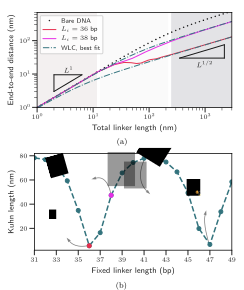
\includegraphics[width=0.48\textwidth]{fig2.png}%
    \caption{(a) Average end-to-end distances for
    homogeneous chromatin chains with \SI{36}{\basepair} and \SI{38}{\basepair} linkers, compared to
    bare DNA and the best-fit WLCs. Rigid rod ($L^1$), Gaussian chain ($L^{1/2}$), and cross-over regimes highlighted.
    (b)
    Kuhn lengths of homogeneous chromatin
    chains are 10.5bp periodic in linker length.
    Example zero-temperature chain
    configurations are shown, including two example Monte Carlo (fluctuating) structures for the \SI{41}{\basepair} case.
    Compact structures (36, \SI{47}{\basepair}) {\color{red}have smaller Kuhn lengths} than less compact structures (\SI{41}{\basepair}).}
    \label{fig:homo-chain}
\end{figure}

%\section{\label{sec:results}Results}

We begin by computing the end-to-end distance $\sqrt{\RR}$ of the
    chain using the formula $\lim_{k\to0} \frac{\partial^{n} B_{000}^{000}}{\partial k^{n}} = i^n \left\langle
    R^n\right\rangle$.
From this, we extract the Kuhn length, $b = \lim_{N\to\infty} \RR/\sum_{i=0}^N L_i$, {\color{red}where a smaller Kuhn length corresponds to a more compact chain. For a WLC, $b=2l_p$ and thus increases with the polymer's stiffness.}

In Fig.~\ref{fig:homo-chain}a, we plot $\sqrt{\RR}$ as a function of chain
    length for homogeneous chains of nucleosomes with \SI{36}{\basepair} and \SI{38}{\basepair}
    linkers. We compare these curves to the $\sqrt{\RR}$ of a TWLC with the same Kuhn length but without kinks.
At short length scales, the slope of $\sqrt{\RR}$ for all chains is one,
    corresponding to rigid-rod behavior.
At the persistence length, the bare WLC's slope smoothly transitions to $1/2$ (on a log-log scale), corresponding to random-walk behavior. In contrast, the homogeneous chain $\sqrt{\RR}$ jumps from that of bare DNA to that of the best-fit WLC, whose Kuhn length is dramatically smaller than twice the persistence length of bare DNA\@.

To build a geometric intuition for how the kinks create this modified Kuhn
    length, we compare the Kuhn lengths of homogeneous, fluctuating chains to their
    zero-temperature configurations, where the entire chain is composed of
    rigid-rod linkers.
Every homogeneous chain at zero temperature forms a helix of nucleosomes.
The rise per basepair of the helix is determined by the spherical angles
    $\theta$ and $\phi$ connecting adjacent linkers (see Fig.~\ref{fig:nuc-geo}).
The nucleosome structure fixes $\theta$, but $\phi$ depends linearly on the
    linker length, and is \SI{10.5}{\basepair}-periodic due to the DNA's helicity.
Select values of $\phi$ lead to more compact zero-temperature structures with a
    smaller rise per basepair.
As seen in Figure~\ref{fig:homo-chain}b, the fluctuating structures with
smaller rise per basepair have smaller Kuhn lengths.

The \SI{10.5}{\basepair} periodicity of $\phi$ as linker length changes leads
    to the periodicity in Figure~\ref{fig:homo-chain}b.
As $L_i\to\infty$, the Kuhn length approaches that of bare DNA only slowly (see Supplemental Material~\cite{supplemental}, Fig.~S4).

\begin{figure}[t]
    \centering
    \includegraphics[width=0.48\textwidth]{fig3.pdf}%
    \caption{Kuhn length of a heterogeneous chromatin chain with uniformly
    distributed linker lengths chosen from the range $\mu \pm \sigma$, where
    $\mu = \SI{41}{\basepair}$. Example zero-temperature chains composed of rigid
    rod linkers are shown for $\sigma = 0, 2, \SI{6}{\basepair}$. Kuhn length
    rapidly approaches that of the exponential chain (black line) in which linker lengths are exponentially distributed about the same $\mu$. }\label{fig:hetero-geom}
\end{figure}

We next consider heterogeneous chains where the linker lengths are drawn uniformly from a
    range $\mu \pm \sigma$.
In Fig.~\ref{fig:hetero-geom}, we see that as we increase $\sigma$, the
    zero-temperature configuration of the chain interpolates between a helix at
    $\sigma = 0$ and a random walk at larger $\sigma$.
As a result, the zero-temperature structure itself has a Kuhn length, which describes the compactness of the random walk.
As in the homogeneous case, the Kuhn length of the zero-temperature chain
    qualitatively predicts that of the fluctuating structure, as seen in
    Fig.~\ref{fig:hetero-geom}.
We find that even a single basepair of variance in nucleosome positions (see e.g.\ Supplemental Material~\cite{supplemental}, Fig.~S5) can create enough geometric stochasticity at zero-temperature to prevent the formation of regular fibers.

\begin{figure}[t]
    \centering
    \includegraphics[width=0.48\textwidth]{fig4.pdf}%
    \caption{Kuhn lengths of chromatin chains with exponentially
    distributed linkers as a function of the average linker length, which
    varies by cell type. Kuhn lengths for \textit{S. cerevisiae}
    ($\meanli=\SI{15}{\basepair}$), mice embryonic stem cells
    (\SI{45}{\basepair}), and human T cells
    (\SI{56}{\basepair}) are labeled.}\label{fig:exp-chain}
\end{figure}


In the simplest model of nucleosome binding, nucleosomes bind uniformly randomly along the DNA~\cite{beshnova2014}, resulting in nucleosome spacings that are exponentially distributed (hereafter ``the exponential chain").
While this picture ignores some details of \textit{in vivo} nucleosome formation, Fig.~\ref{fig:hetero-geom} shows how any linker length distribution with sufficiently large variance ($\sigma$) will exhibit behavior similar to the exponential chain.
Thus, the results that follow are likely robust to adding more detail to the nucleosome binding model.

When averaged over the distribution of possible nucleosome
    positions, the end-to-end distance of our exponential chain takes the form of a WLC with a rescaled Kuhn length (see Supplemental Material~\cite{supplemental},
    Fig.~S6).
This makes sense because at zero temperature our model differs from a freely rotating chain only in the correlation between linker length and $\phi$, and the freely rotating chain is known to converge to a wormlike chain under
    appropriate scaling~\cite{kilanowski2017}.
We extract the rescaled Kuhn length as a function of $\meanli$ in
    Fig.~\ref{fig:exp-chain}.

Unlike the homogeneous case, where changing $L_i$ selects between zero-temperature helices,
    increasing $\meanli$ in the heterogeneous case scales the zero-temperature random walk.
As a result, Fig.~\ref{fig:exp-chain} lacks
    the \SI{10.5}{\basepair} periodicity of the homogeneous chain.
Thus, for the purposes of coarse-graining, an approximate knowledge of $\meanli$ should be sufficient to capture chromatin's average behavior as a WLC.
A table of these Kuhn lengths is available in the Supplemental Material~\cite{supplemental}, Table~S1.

\begin{figure}[t]
    \centering
    \includegraphics[width=0.48\textwidth]{fig5.pdf}%
    \caption{Looping probabilities as a function of genomic separation for exponential chains. Each purple line designates an individual chain with linker lengths drawn from an exponential distribution with $\mu = \SI{56}{\basepair}$. The red shaded area corresponds to 95\% confidence intervals around the mean over the individual chains (red line). A wormlike chain
    (black dashed line) with the same Kuhn length as this average chain captures the
    looping probability for loops with at least three intervening nucleosomes. Three
    random individual chains are bolded.\label{fig:looping}}
\end{figure}

    To characterize the chain's {\color{red}structure} on shorter length scales, we calculate the
    probability of genomic contacts (\emph{i.e.} the looping probability).
By numerically inverting the Fourier transform in Eq.~\ref{eq:expansion}, we
    can analytically evaluate $P_\text{loop}=\greens[L]{\vec{R}=0}$, a
    modified $J$-factor with no orientational component.
In Fig.~\ref{fig:looping}, we plot this probability as a function of the loop size.

Strikingly, we observe that for a fixed genomic separation, different nucleosome
spacings can change the contact probability by up to six orders of magnitude.
The average looping probability, which is relevant at
    timescales where nucleosome positions can re-randomize, is captured well by a single
    WLC.
Due to this effective WLC's reduced Kuhn length, we predict that chromatin's propensity for forming
    sub-kilobase-scale loops should be one to four orders of magnitude larger than that of bare DNA.
The predicted looping propensity peaks at a length scale typical of promoter contacts \textit{in vivo}
    and consistent with Hi-C looping data~\cite{sanborn2015} (see Supplemental
    Material~\cite{supplemental}, Fig.~S8).
This result highlights how even without models of DNA more detailed than the
WLC---for example those including DNA
melting~\cite{shimada1984,liu2011a,wiggins2005}---the propensity of small DNA
loops can be enhanced by proteins that promote stochastically spaced kinks in the DNA.

Additionally, we find that the average looping probability is higher than that of most of the individual chains.
Thus, even an ``informationless'' chromatin remodeler that merely promotes random
    nucleosome repositioning will greatly facilitate sub-kilobase loop formation.
At longer length scales, the looping probabilities approach the characteristic $L^{-3/2}$
    Gaussian scaling.
However, individual chains retain memory of their kinks, as indicated by
    how the highlighted chains persist above or below the average.
Using a uniform linker length distribution
    leads to qualitatively similar results (see Supplemental Materials~\cite{supplemental}, Fig.~S9).


In conclusion, we provide rigorous justification for using
    an effective WLC to model \textit{in vivo} chromatin. Due to the lack of experimental consensus on the persistence length $l_p$ of chromatin~\cite{langowski2006a},  coarse-grained models of chromatin have historically used a range of values for $l_p$, sometimes even just using that of bare DNA~\cite{benedetti2017,macpherson2018,nuebler2018}.
We show that this choice leads to at least a
    two-fold overestimation of the polymer's {\color{red}persistence length}
    %a concomitant underestimation of the looping probabilities at long length scales,
    and a
    several orders-of-magnitude underestimation of looping at short length scales.
Some past models have extracted a parameter that describes the linear compaction of
    chromatin (bp per nm of fiber) from Hi-C looping probabilities
    (see e.g.~\cite{ghosh2018, rosa2008}).
Our model's parameter-free estimate of chromatin's {\color{red}looping propensity} provides a theoretical explanation for the effective
    Kuhn length predicted from these experimental measurements.


% \section{\label{sec:discussion}Discussion}

Our model excludes various important facets of chromatin's structure, such as
    interaction energies (sterics and stacking) and nucleosome ``breathing''.
Since nucleosome breathing simply corresponds to choosing a different distribution for the angle $\theta \in [0, \pi]$
    between adjacent nucleosomes, incorporating breathing leaves our results qualitatively unchanged (see Supplemental Material~\cite{supplemental}, Fig.~S10).
However, a more careful inclusion of breathing will likely require an explicit treatment of the
    effects of DNA sequence and linker histone on the nucleosome particle.


Our work highlights that the geometric effects of heterogeneous nucleosome binding
    dominate thermal fluctuations {\color{red}in driving chromatin contacts} \textit{in vivo}.
Our insights into chromatin's {\color{red}stiffness} will also inform future studies on the effects of
    loop extrusion factors~\cite{nuebler2018,brackley2017} and epigenetic
    states~\cite{macpherson2018,michieletto2016,brackley2017}
    on chromatin organization.\@

\begin{acknowledgements}
Financial support for this work is provided by the National Science Foundation
    (NSF), Physics of Living Systems Program (PHY-1707751). Q.M. and B.B.
    acknowledge funding support from the NSF Graduate Fellowship program
    (DGE-1656518). B.B. acknowledges support from NIH Training Grant
    T32GM008294.
\end{acknowledgements}

\bibliography{chromatin}

\end{document}
